\documentclass{beamer}
\usetheme{Madrid}
\usecolortheme{default}
\usepackage{comment}

\title[Random Vectors ]
{Random Vectors\newline }

\subtitle{}

\author[Mohadeseh Shafiei Kafraj] % (optional, for multiple authors)
{Mohadeseh Shafiei Kafraj\inst{1}}

%{A.~B.~Arthur\inst{1} \and J.~Doe\inst{2}}

\institute[UCL] % (optional)
{
  \inst{1}%
  Gatsby Computational Neuroscience Unit\\
  University College London
  %\and
  %\inst{2}%
  %Faculty of ...\\
  %University...
}

\date[Gatsby Bridging Programme  2023] % (optional)
{Gatsby Bridging Programme 2023}

\logo{
\includegraphics[height=0.8cm]{GATSBY_Logo.jpg}}

\definecolor{uoftblue}{RGB}{6,41,88}
\setbeamercolor{titlelike}{bg=uoftblue}
\setbeamerfont{title}{series=\bfseries}

\begin{document}

\frame{\titlepage}

\begin{frame}
\frametitle{Table of Contents}
\tableofcontents
\end{frame}


%1
\section{PDF and CDF}
\begin{frame}
This slide requires a change:
\frametitle{Random Vectors: When are they useful?}
\center 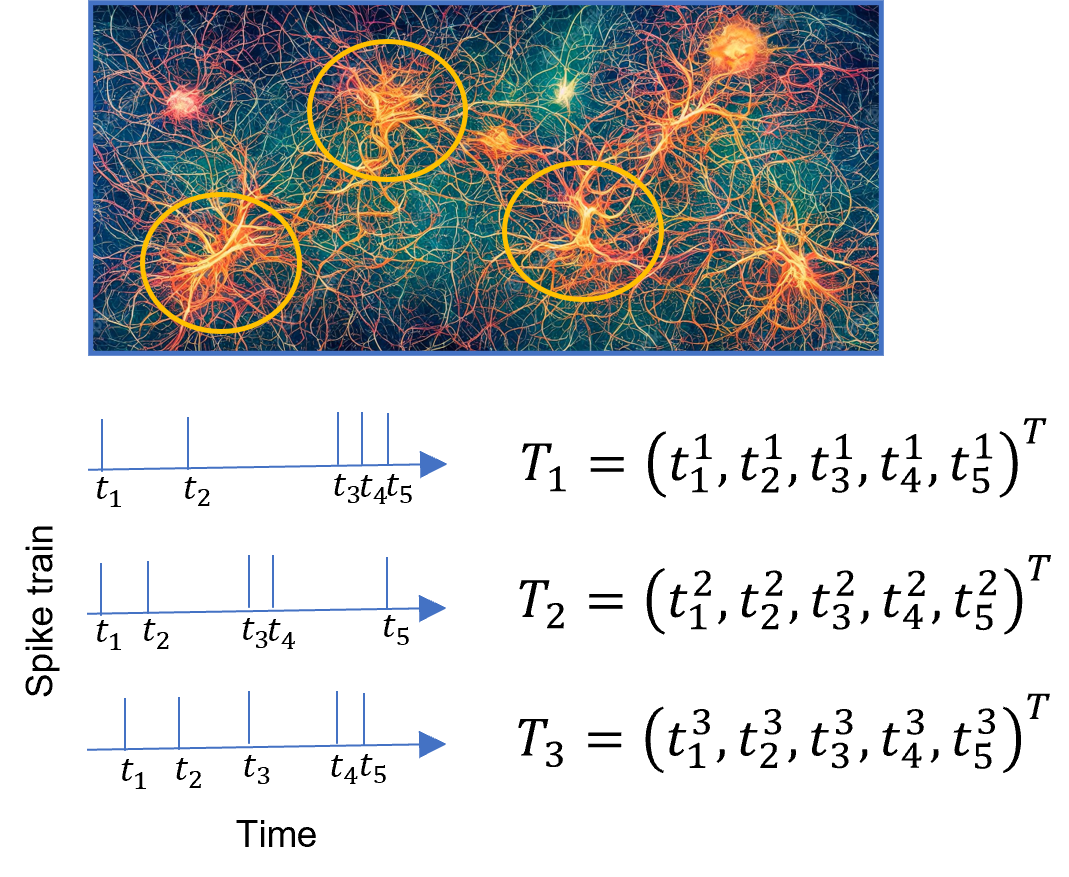
\includegraphics[height=6cm]{Random_Vector_Example.png}
\end{frame}

%2
\begin{frame}
\frametitle{PDF and CDF}
$X = (X_1, ..., X_n)^T$: A random vector\newline \\
$F_x(x)$: *Cumulative* Distribution Function(*CDF*)\newline\\
$f_x(x)$: Probability *Density* function (*pdf*)\newline\\
\end{frame}

%3
\begin{frame}
\frametitle{PDF and CDF}
By definition, Cumulative Distribution Function(CDF) is:\newline
$F_x(x) = P[X_1 \le x_1, ..., X_n\le x_n]$\newline\\
$x = (x_1, ..., x_n)$ we get:\newline\\
$F_x(x) = P[X\le x]$\newline\\
we associate the events:\newline
${X \le \infty}$ with the certain event, $F_x(\infty) = 1$,and\newline\\
${X \le -\infty}$ with the impossible event, $F_x(-\infty) = 0.$\\
\end{frame}

%4
\begin{frame}
\frametitle{PDF and CDF}
The probability *density* function (pdf) is defined as:\newline\\
$f_x(x) = \frac{\partial^n{F_x(x)}}{\partial{x_1}...\partial{x_n}}$\newline\\
Equivalently we could have defined it as:\newline\\
$f_x(x) = {\lim_{\Delta x_1 \to 0,...,\Delta x_n \to 0} \frac{P[x_1<X_1\le x_1+\Delta x_1,...,x_n<X_n\le x_1+\Delta x_n]}{\Delta x_1...\Delta x_n}}$\newline\\
Therefore, \newline\\
$f_x(x) \Delta x_1...\Delta x_n \simeq {P[x_1<X_1\le x_1+\Delta x_1,...,x_n<X_n\le x_1+\Delta x_n]}$\newline\\
\end{frame}

%7
\begin{frame}
\frametitle{PDF and CDF}
pdf is defined as:\newline\\
$f_x(x) = \frac{\partial^n{F_x(x)}}{\partial{x_1}...\partial{x_n}}$\newline\\
if we integrate the equation, we obtain:\newline\\
$F_x(x) = \int_{-\infty}^{x_1}...\int_{-\infty}^{x_n} f_x(x^{'})dx_1^{'}...dx_n^{'} = \int_{-\infty}^{x} f_x(x^{'})dx^{'}$\newline\\
more generally:\newline\\
$P [B] = \int_{x \in B} f_x(x^{'})dx^{'} $, where $B \subset R^N$
\end{frame}

%8
\begin{frame}
\frametitle{PDF and CDF}
constraint: $(P[B]\neq 0)$\newline\\
conditional *CDF*: $F_{x|B}(x|B) = P[X\le x|B] = \frac{P[X\le x,B]}{P[B]}$  \newline\\

mixture *CDF*: $F_x(x) = \sum _{i=1}^{n} F_{x|B_i}(x|B_i)P[B_i]$ \newline\\
conditional *pdf*: $f_{x|B}(x|B)=\frac{\partial^n{F_{x|B}(x|B)}}{\partial{x_1}...\partial{x_n}}$ \newline\\
mixture *pdf*:$f_x(x) =\sum _{i=1}^{n} f_{x|B_i}(x|B_i)P[B_i]$\newline\\
mixture: a linear combination
\end{frame}

%9
\begin{frame}
\frametitle{PDF and CDF}
Joint distribution of *two* random vectors:\newline\\
$X= (X_1,...,X_n).T$\newline\\
$Y = (Y_1,...,Y_M).T$\newline\\
$F_{XY}(x,y) = P[X\le x,Y\le y]$\newline\\
joint density: $f_{XY}(x,y) = \frac{\partial^{n+m}F_{XY}(x,y)}{\partial{x_1}...\partial{x_n}\partial{y_1}...\partial{y_m}}$\newline\\
marginal density: $f_x(x)=\int_{-\infty}^{\infty}...\int_{-\infty}^{\infty} f_{XY}(x,y)dy_1...dy_n $\newline\\

\end{frame}



%2D
\begin{frame}
\frametitle{PDF and CDF: Here's a fun example!}
pdf: $f_x (x) = \frac{exp(-\frac{1}{2}(x-\mu)^T\Sigma^{-1} (x-\mu))}{\sqrt{{2\pi}^k|\Sigma|}}$, \newline\\
where in this example,\newline\\
$ X=[x,y]$, therefore,\newline\\
CDF: $=F_{[x,y]}([x,y]) = \int_{-\infty}^{x}\int_{-\infty}^{y} f_x(x^{'},y^{'})dx^{'}dy^{'} $\newline\\

Step 1:
For this interesting distribution, implement step 1 to see what pdf and CDF look like, for different mean vector and covariance matrices!
\end{frame}

\begin{frame}
\frametitle{PDF and CDF: 2D}
Step1 :
\\mean, $\mu = [0,0]$,\\
covariance matrix $\Sigma = \begin{bmatrix}
    1 & 0 \\
    0&1
\end{bmatrix}$\newline\\
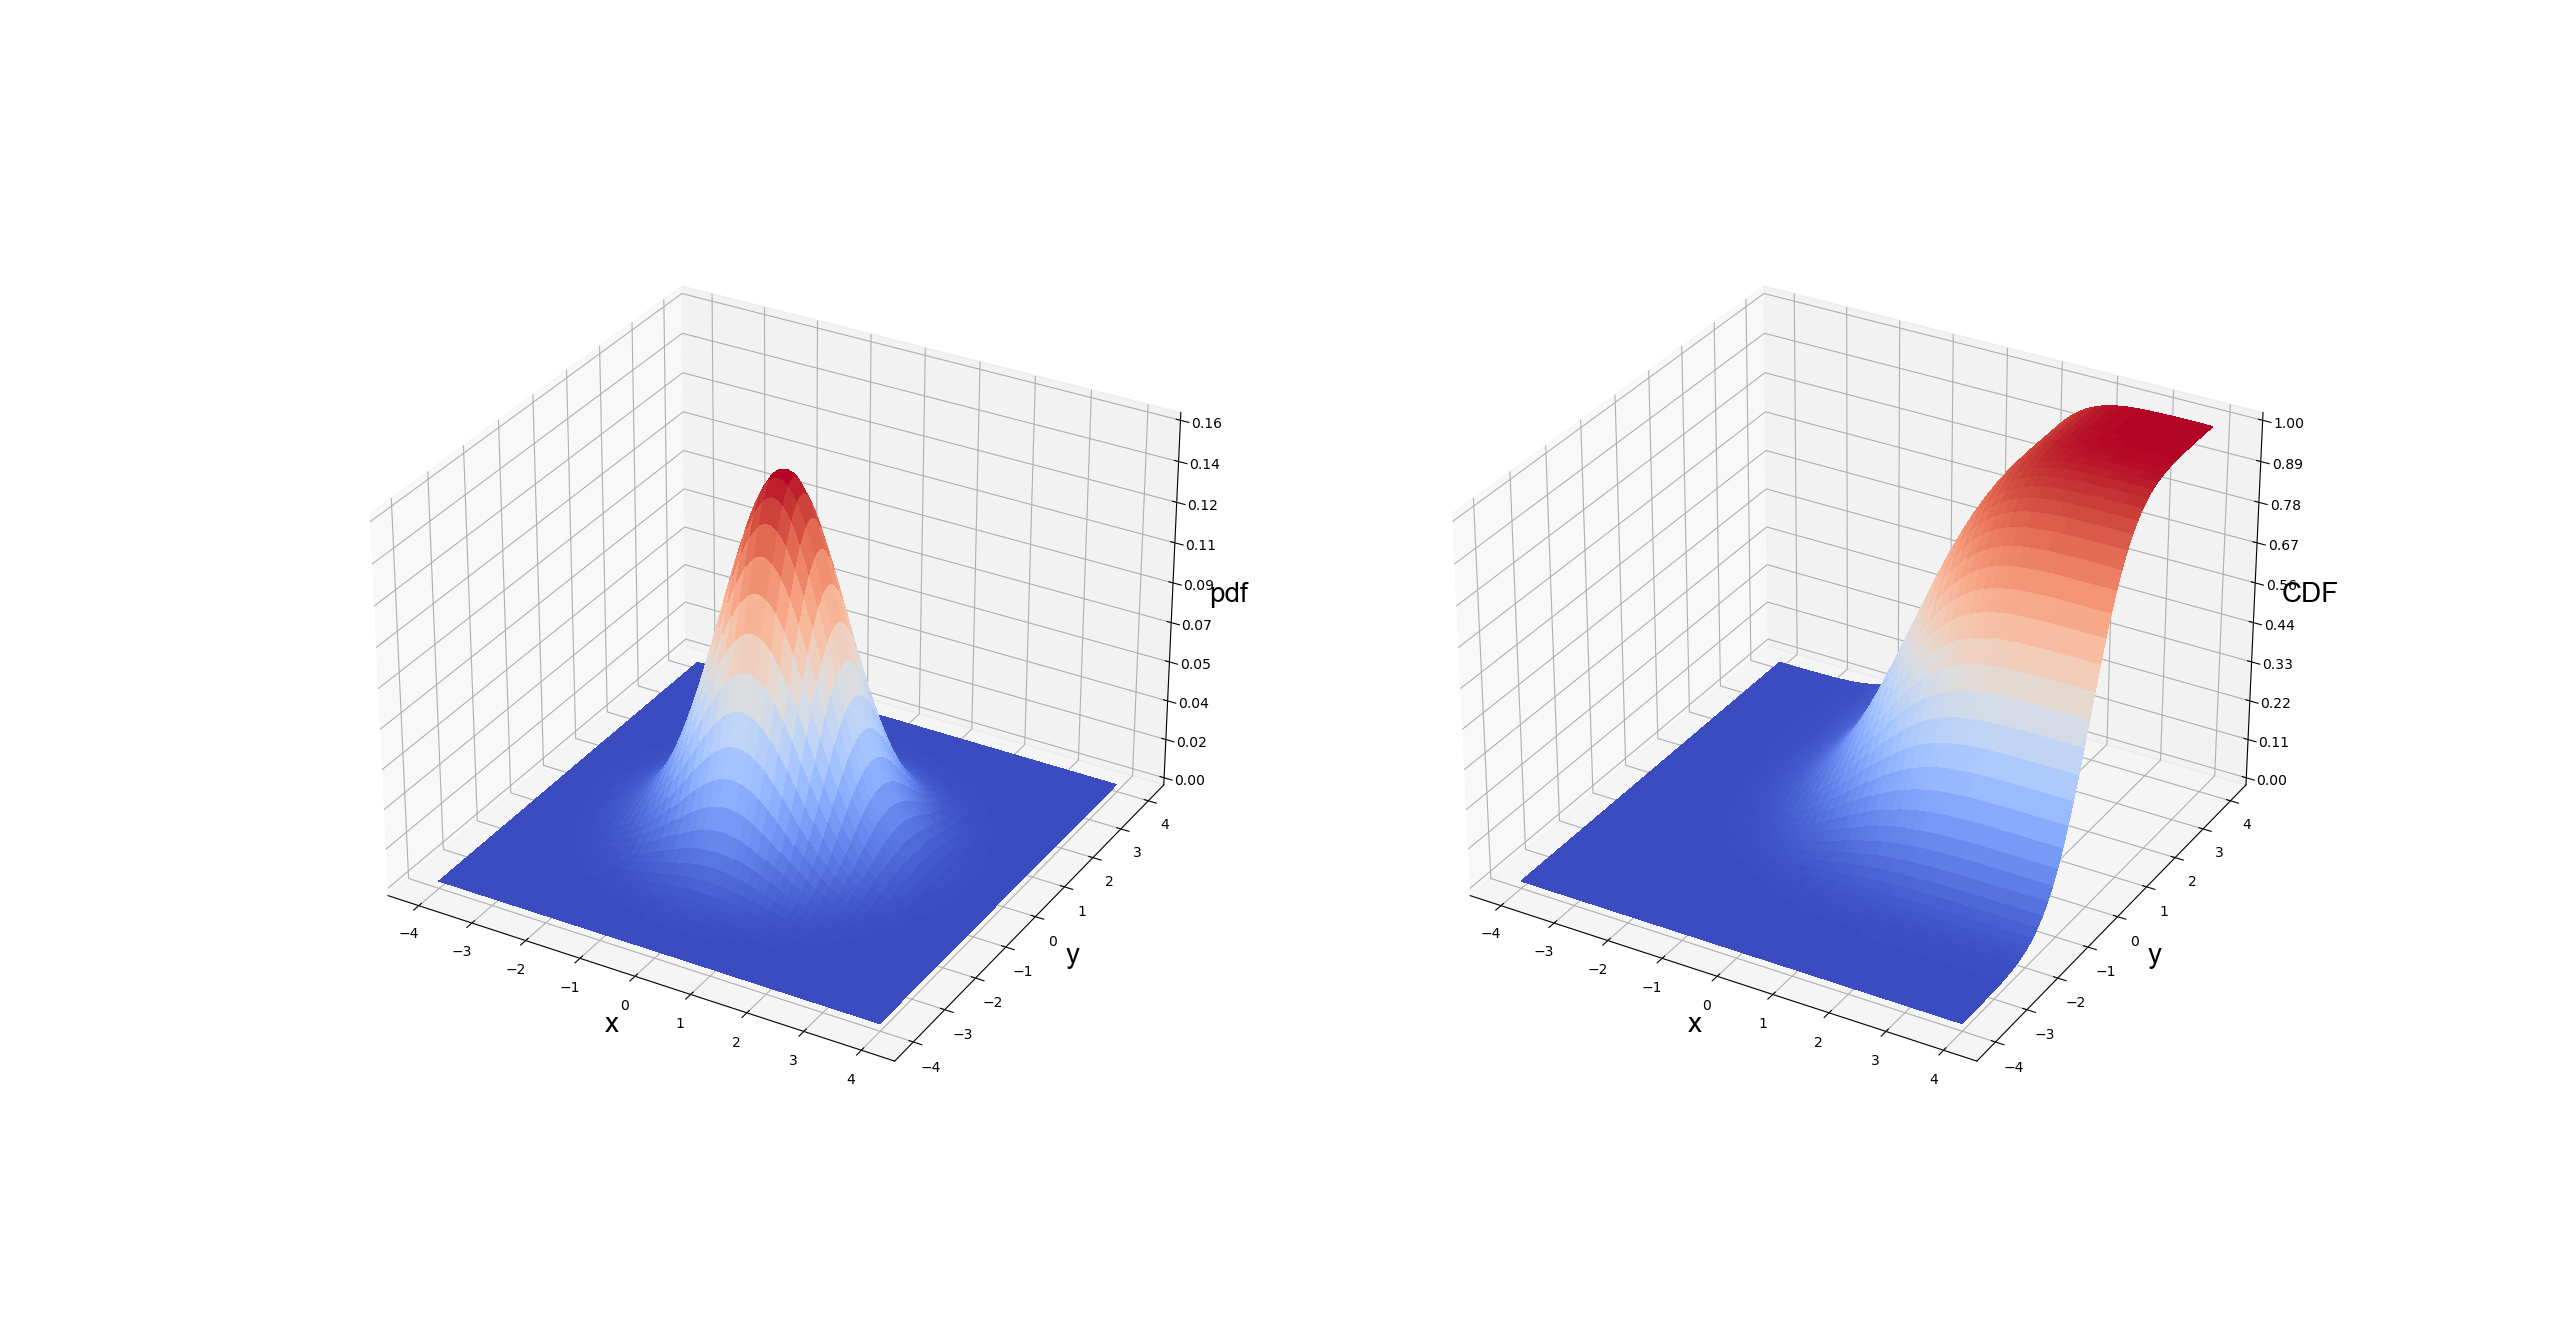
\includegraphics[height=6.5cm]{2D-1.png}
\end{frame}

\begin{frame}
\frametitle{PDF and CDF: 2D}
Step1 :
\\mean, $\mu = [1,0]$,\\
covariance matrix $\Sigma = \begin{bmatrix}
    1 & 0 \\
    0&4
\end{bmatrix}$\newline\\
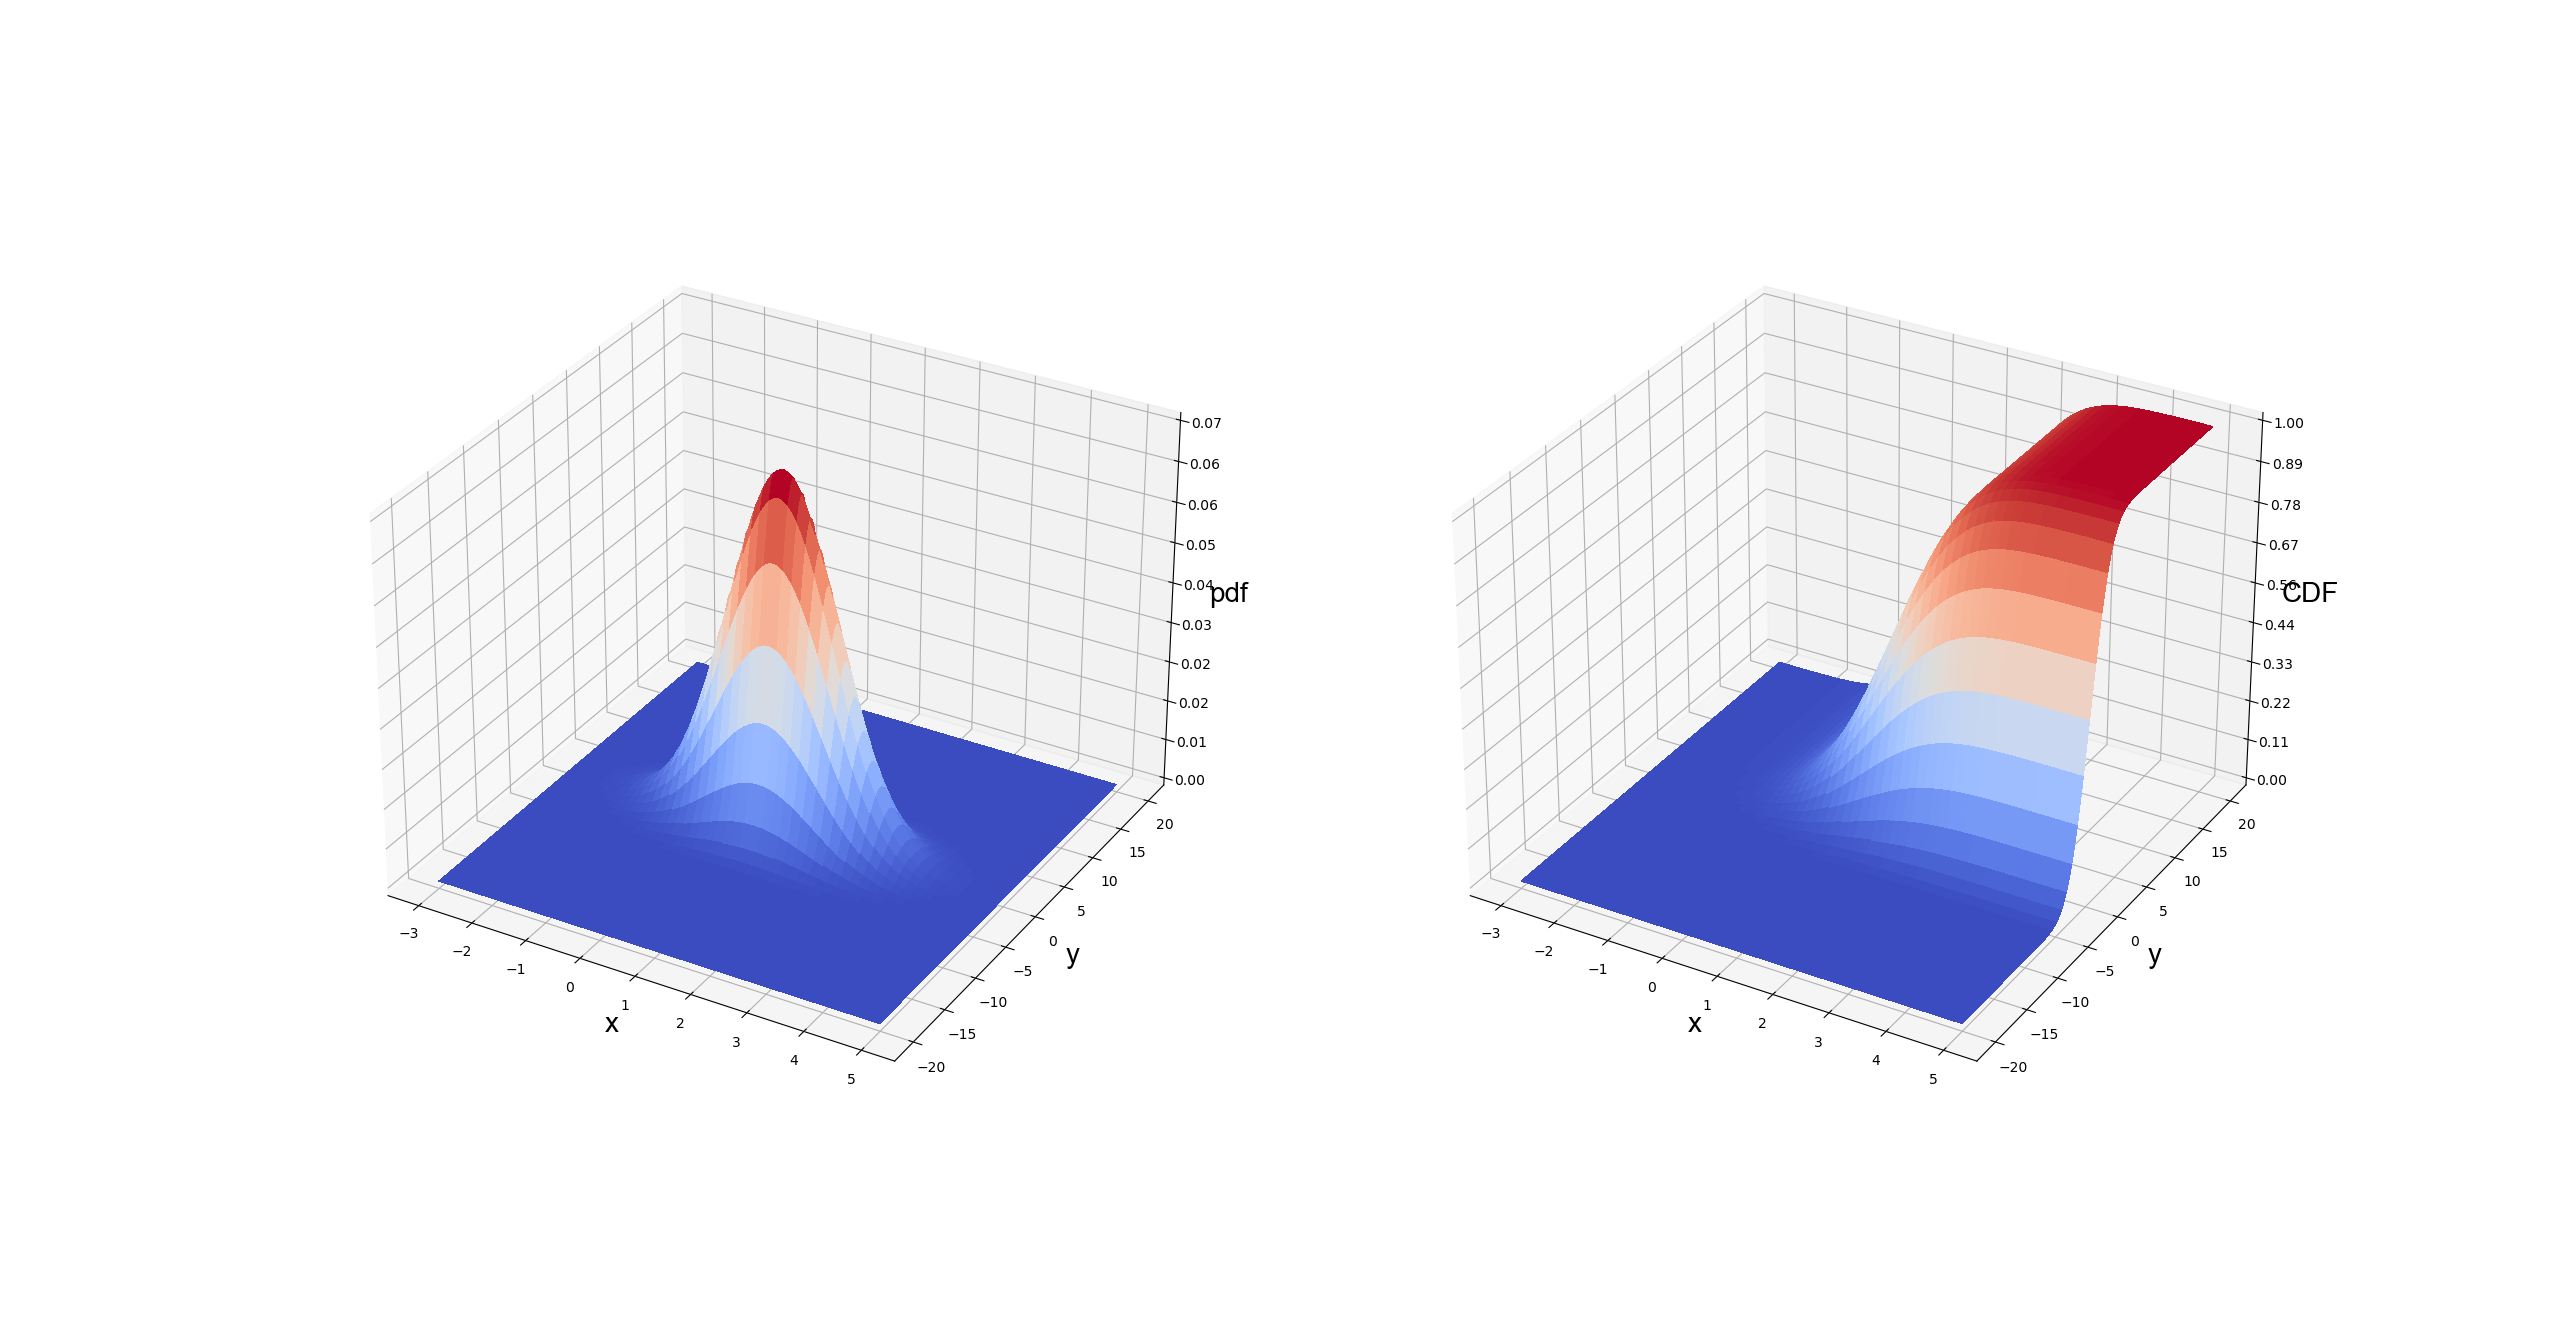
\includegraphics[height=6.5cm]{2D-2.png}
\end{frame}

\begin{frame}
\frametitle{PDF and CDF: 2D}
Step1 :
\\mean, $\mu = [0,0]$,\\
covariance matrix $\Sigma = \begin{bmatrix}
    9 & -8\\
    -8&9
\end{bmatrix}$\newline\\
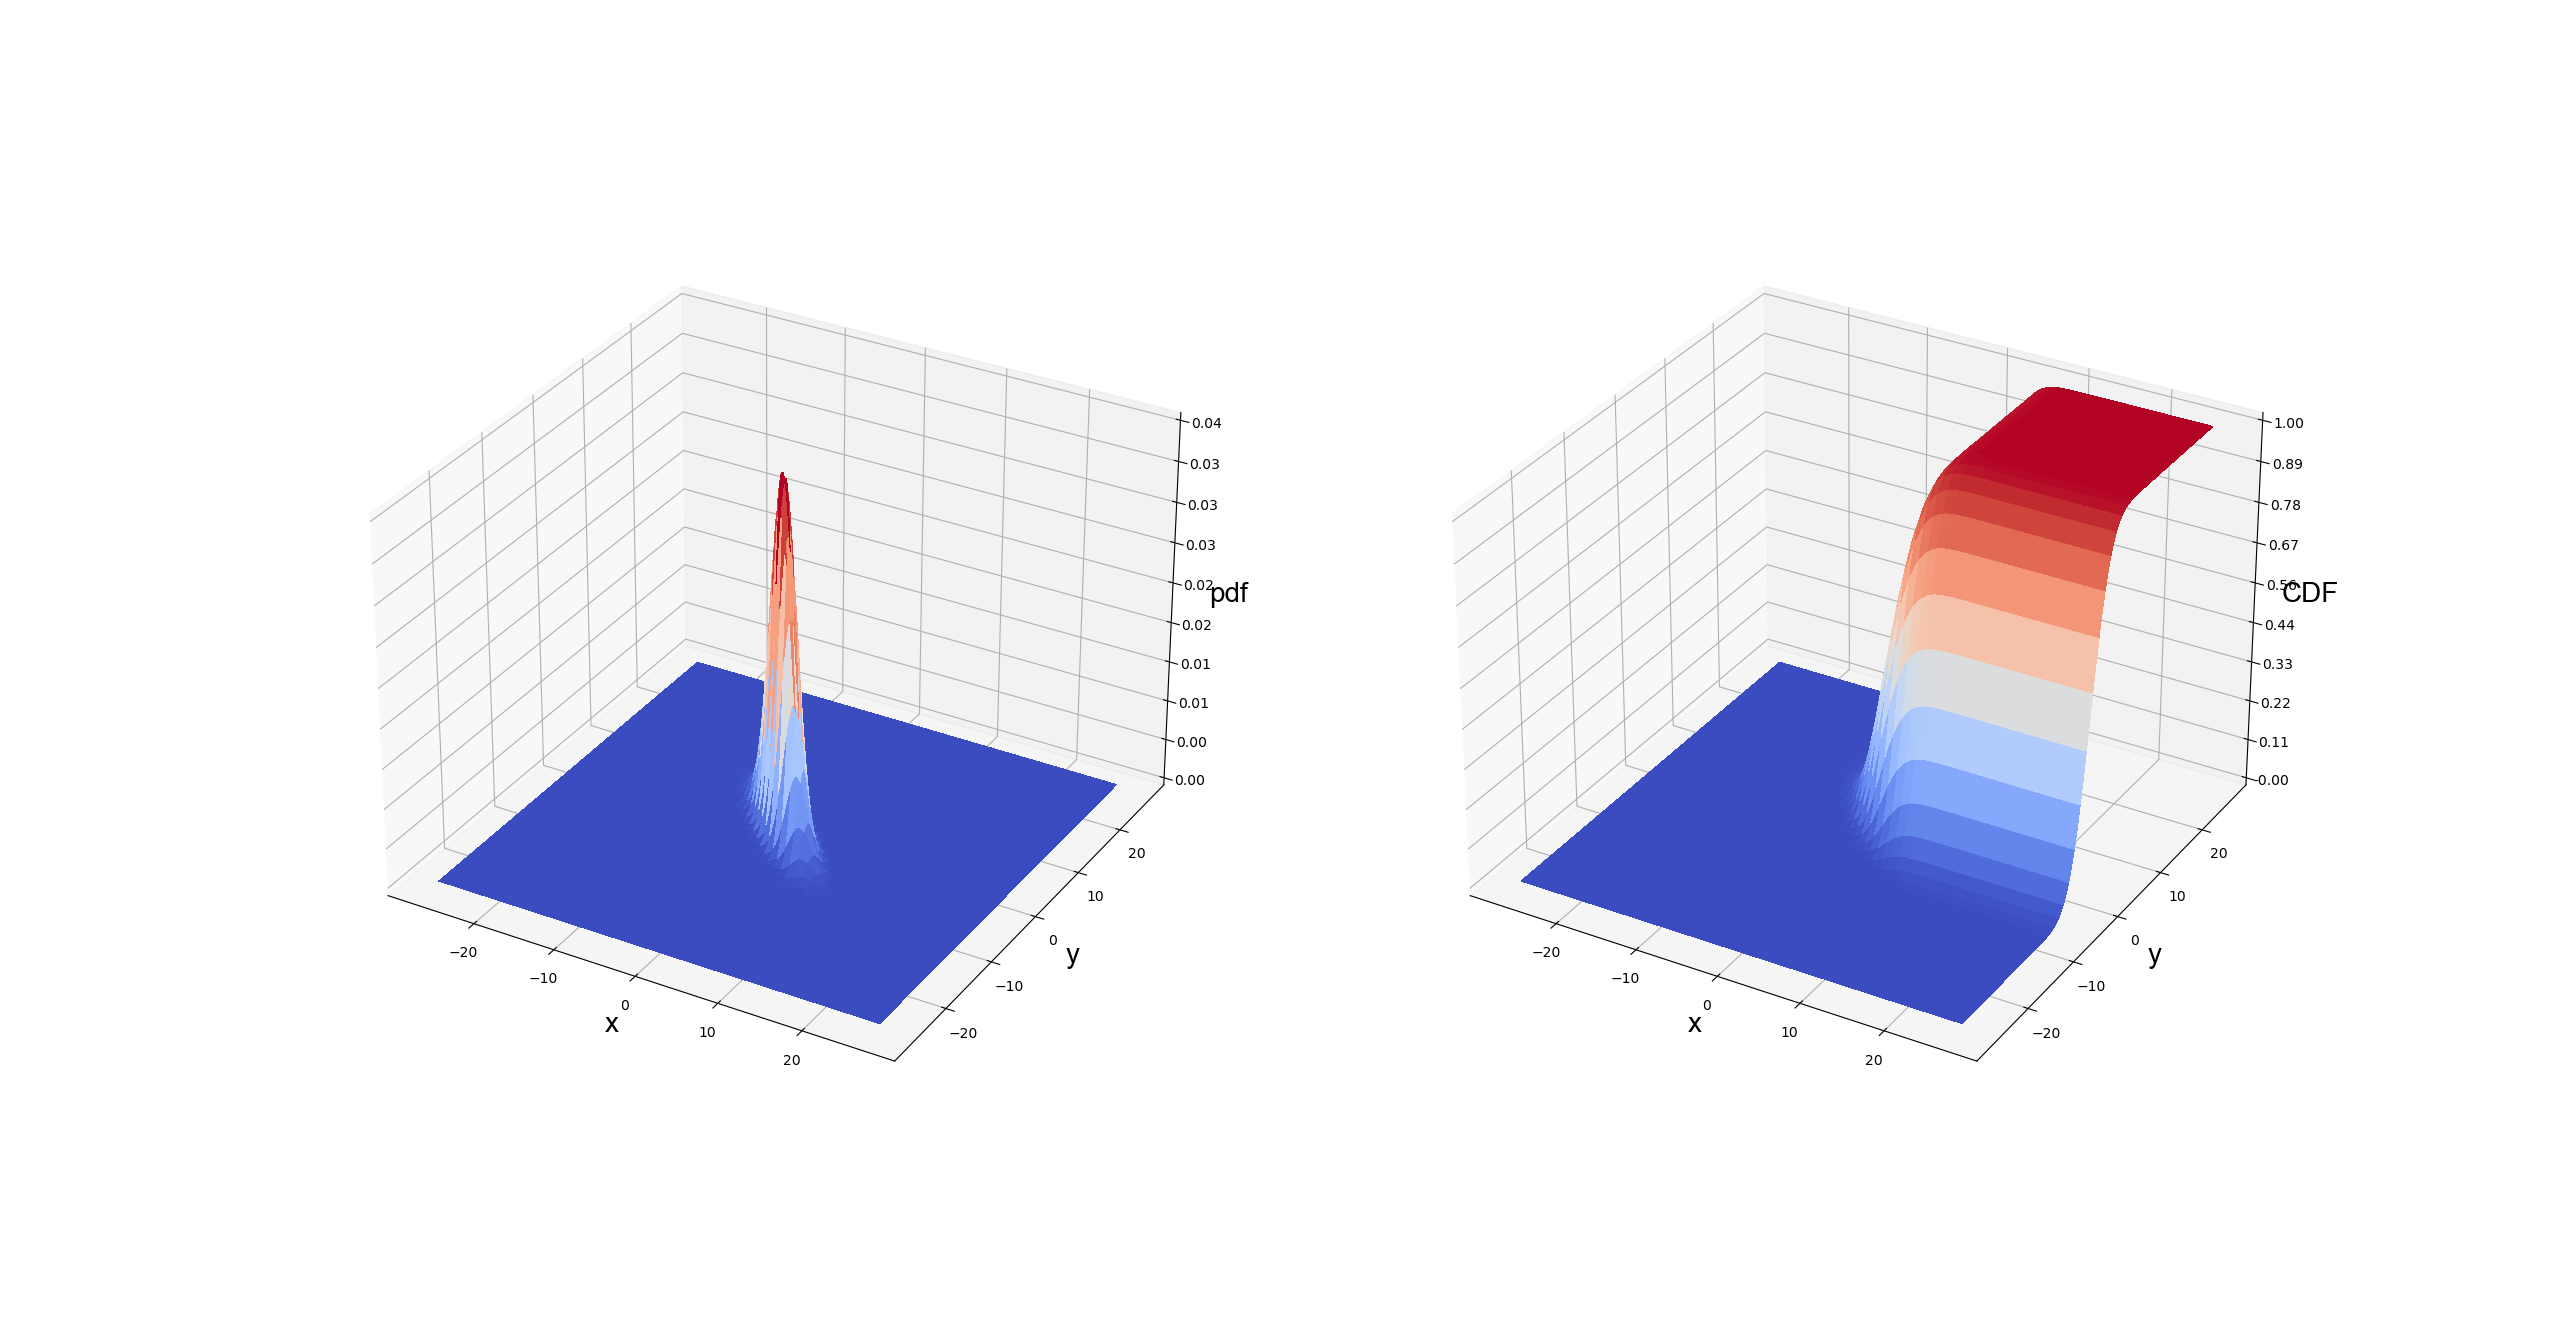
\includegraphics[height=6.5cm]{2D-3.png}
\end{frame}

%3D
\begin{frame}
\frametitle{PDF and CDF: 3D}
pdf: $f_x (x) = \frac{exp(-\frac{1}{2}(x-\mu)^T\Sigma^{-1} (x-\mu))}{\sqrt{{2\pi}^k|\Sigma|}}$, \newline\\
where in this example,\newline\\
$ X=[x,y,z]$, therefore,\newline\\
CDF: $=F_{[x,y,z]}([x,y,z]) = \int_{-\infty}^{x}\int_{-\infty}^{y}\int_{-\infty}^{z} f_x(x^{'},y^{'},z^{'})dx^{'}dy^{'}dz^{'} $\newline\\

Step 2:
Implement step 2 to see what pdf and CDF look like, for different mean vector and covariance matrices!
\end{frame}

\begin{frame}
\frametitle{PDF and CDF: 3D}
Step2 :
\\mean, $\mu = [0,0,0]$,\\
covariance matrix $\Sigma = \begin{bmatrix}
    1 & 0&0 \\
    0&1&0\\
    0&0&1
\end{bmatrix}$\newline\\
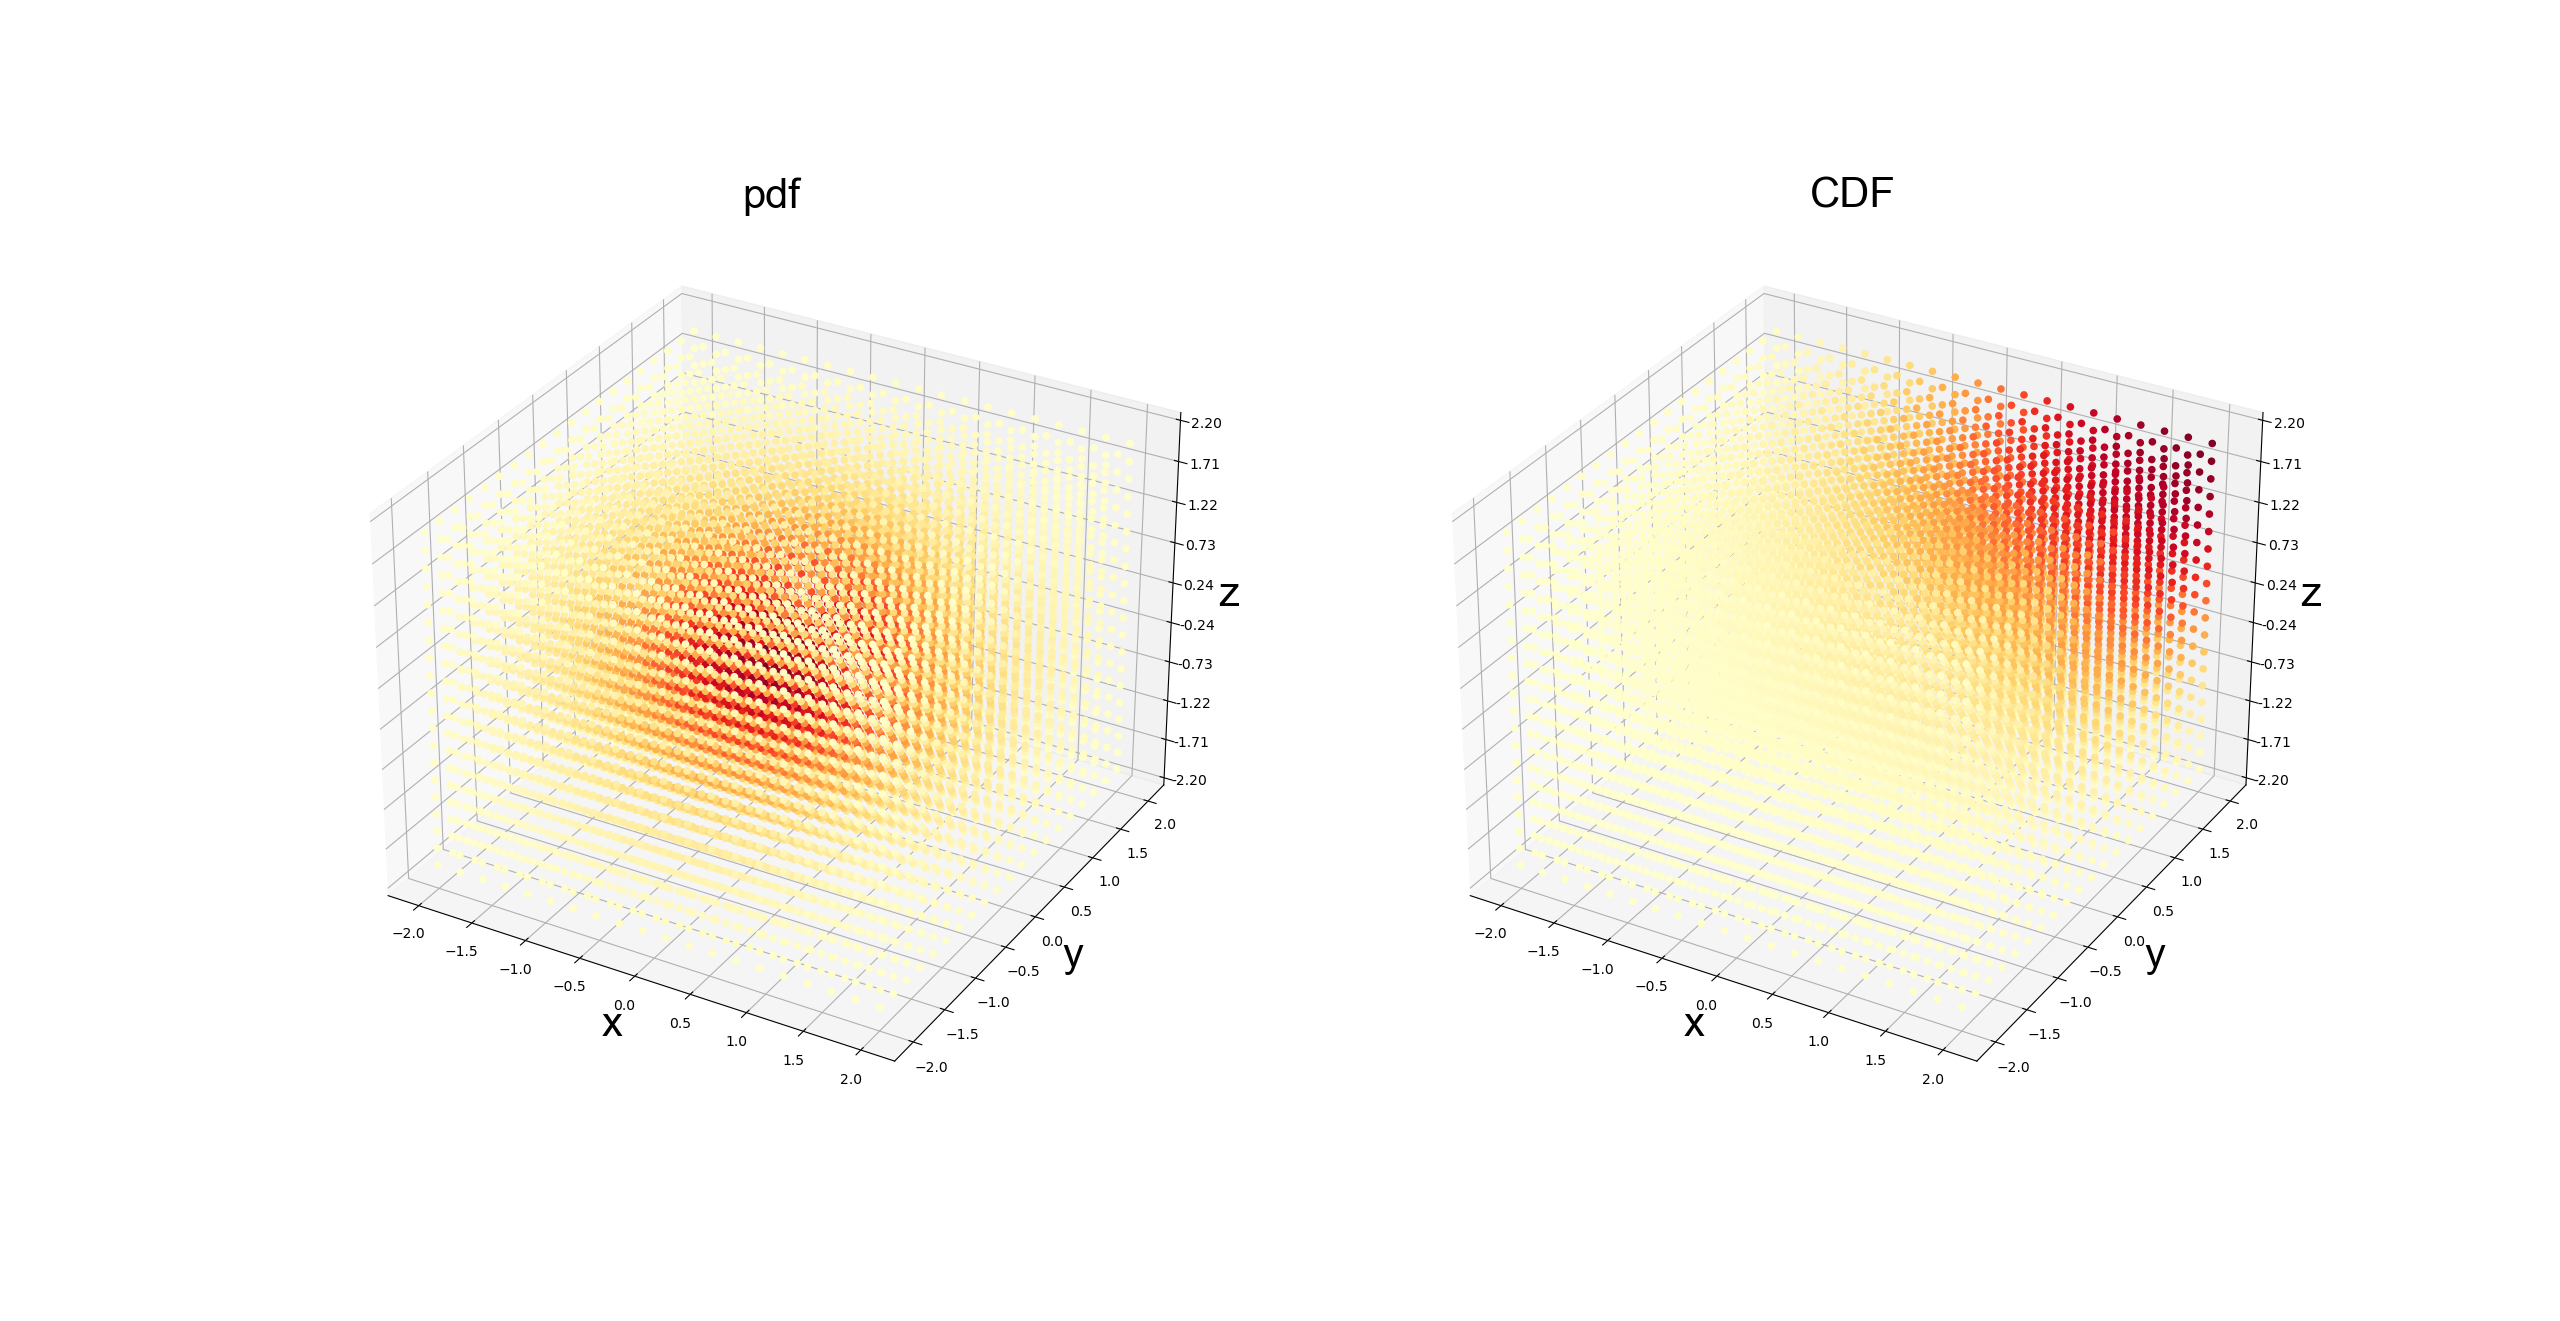
\includegraphics[height=6.5cm]{3D-1.png}
\end{frame}

\begin{frame}
\frametitle{PDF and CDF: 3D}
Step2 :
\\mean, $\mu = [1,1,1]$,\\
covariance matrix $\Sigma = \begin{bmatrix}
    1 & 0&0 \\
    0&3&0\\
    0&0&5
\end{bmatrix}$\newline\\
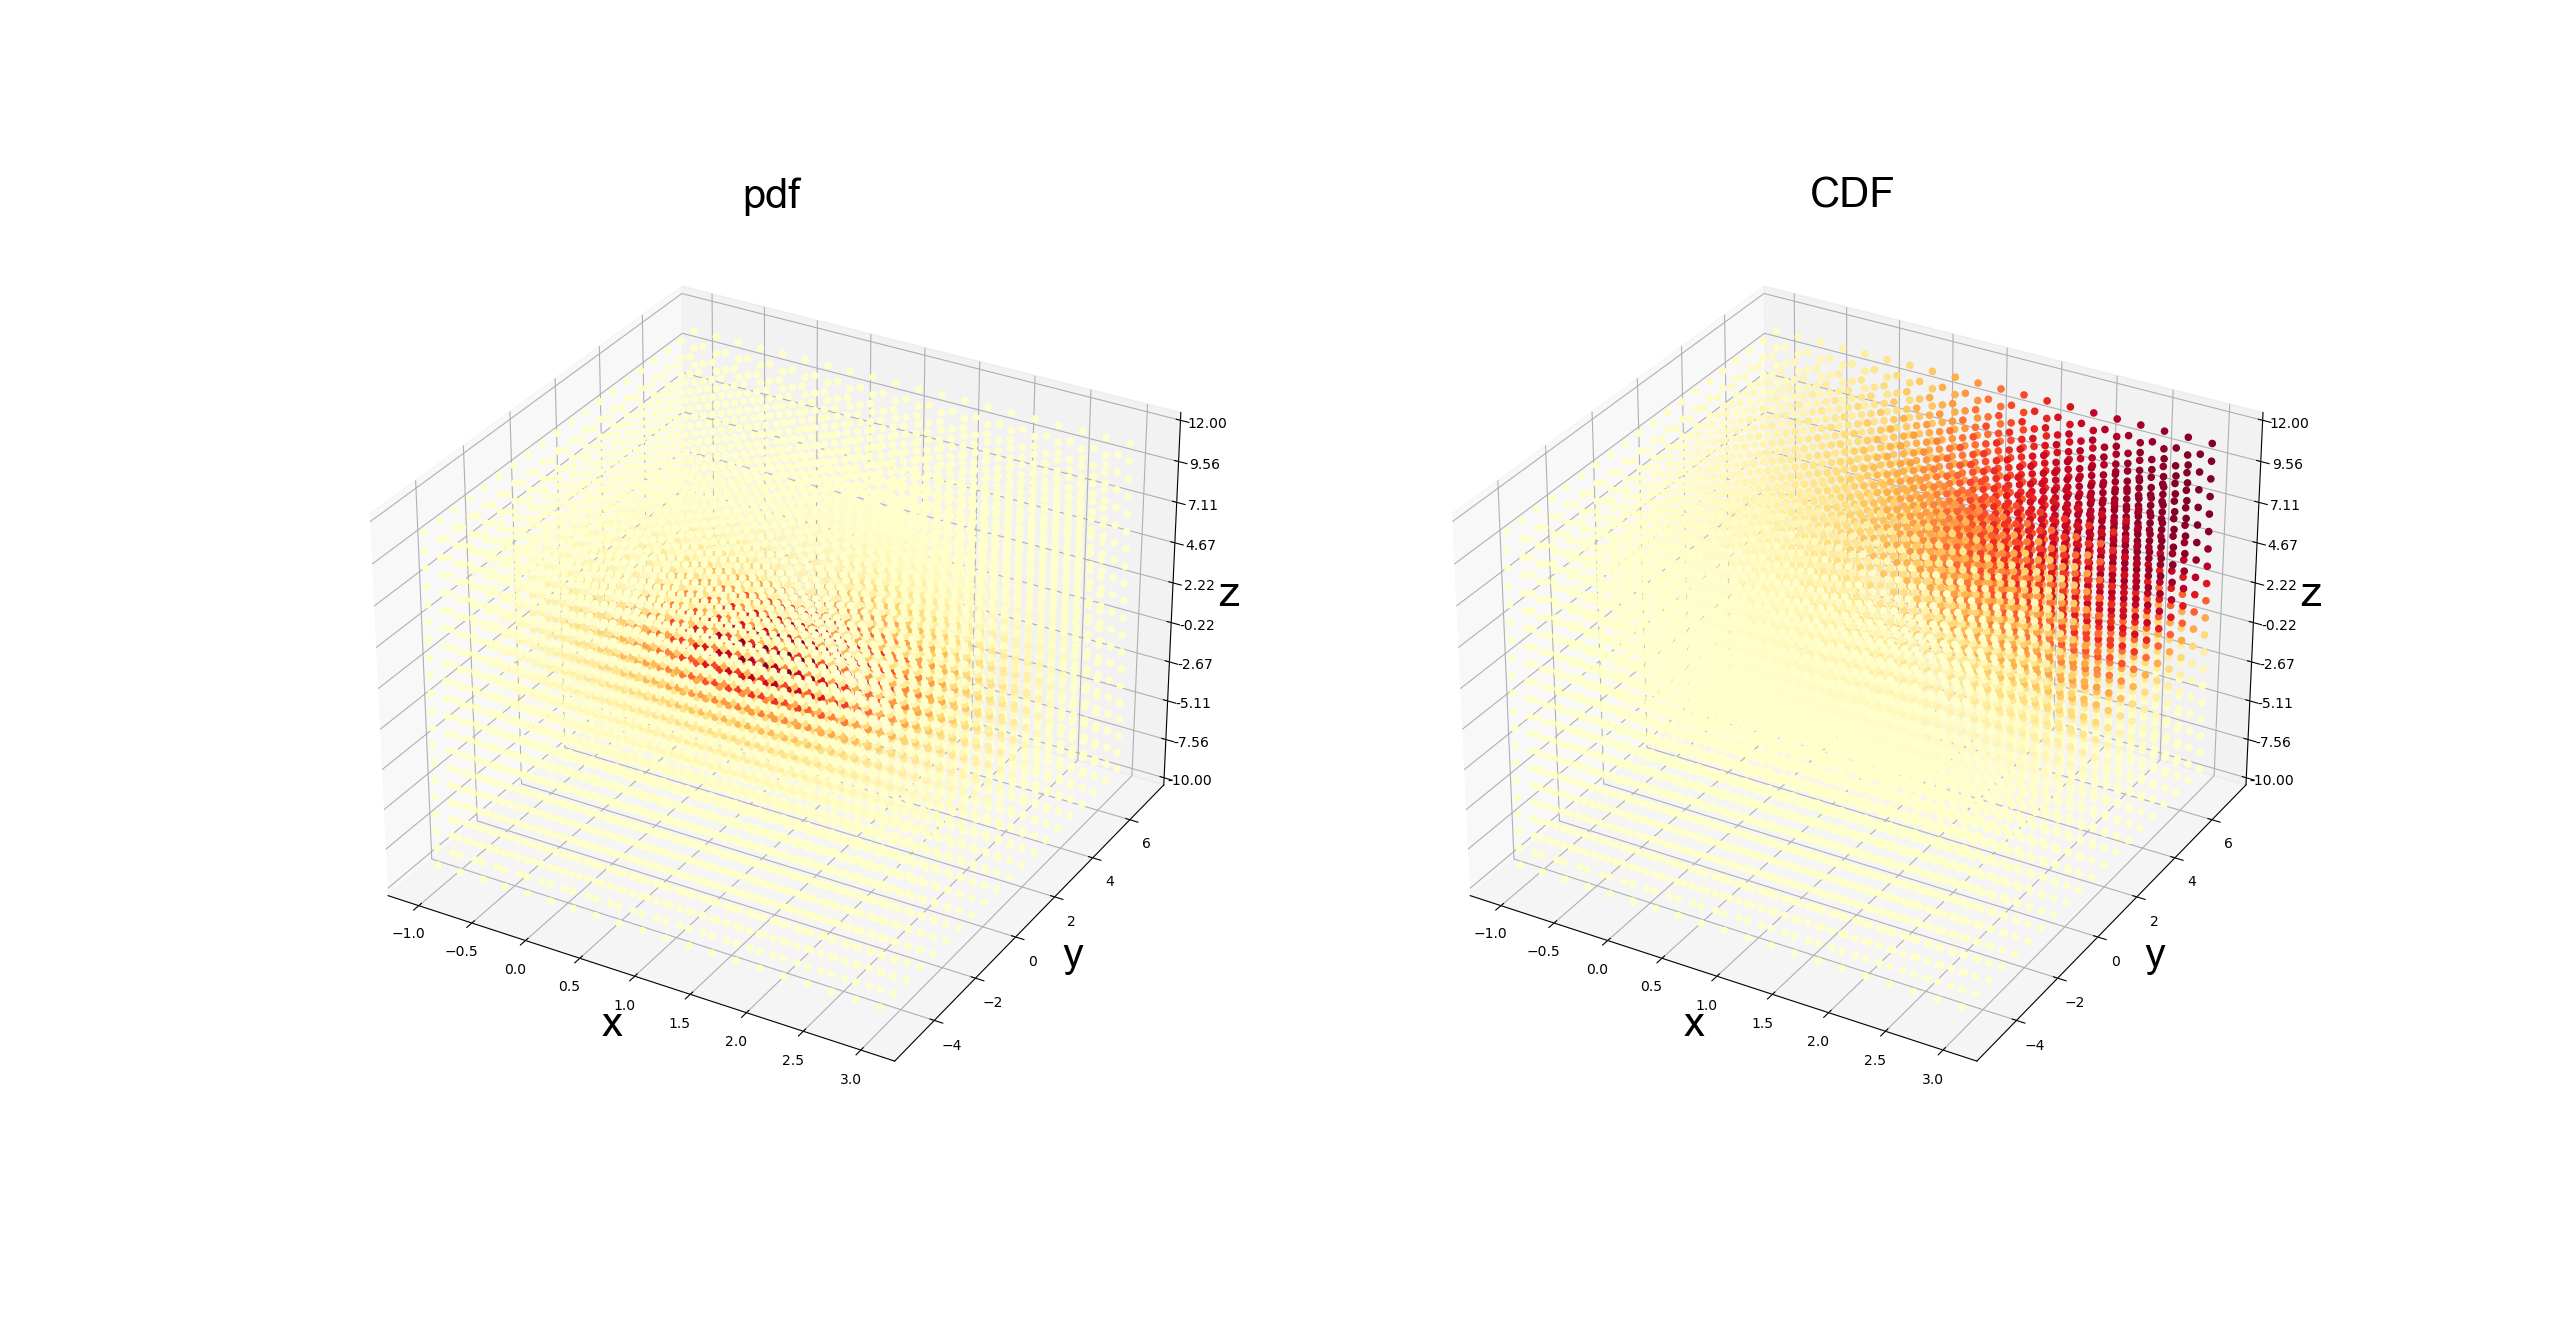
\includegraphics[height=6.5cm]{3D-2.png}
\end{frame}

\begin{frame}
\frametitle{PDF and CDF: 3D}
Step2 :
\\mean, $\mu = [0,0,0]$,\\
covariance matrix $\Sigma = \begin{bmatrix}
    3 & 2&-2 \\
    2&3&0\\
    -2&0&3
\end{bmatrix}$\newline\\
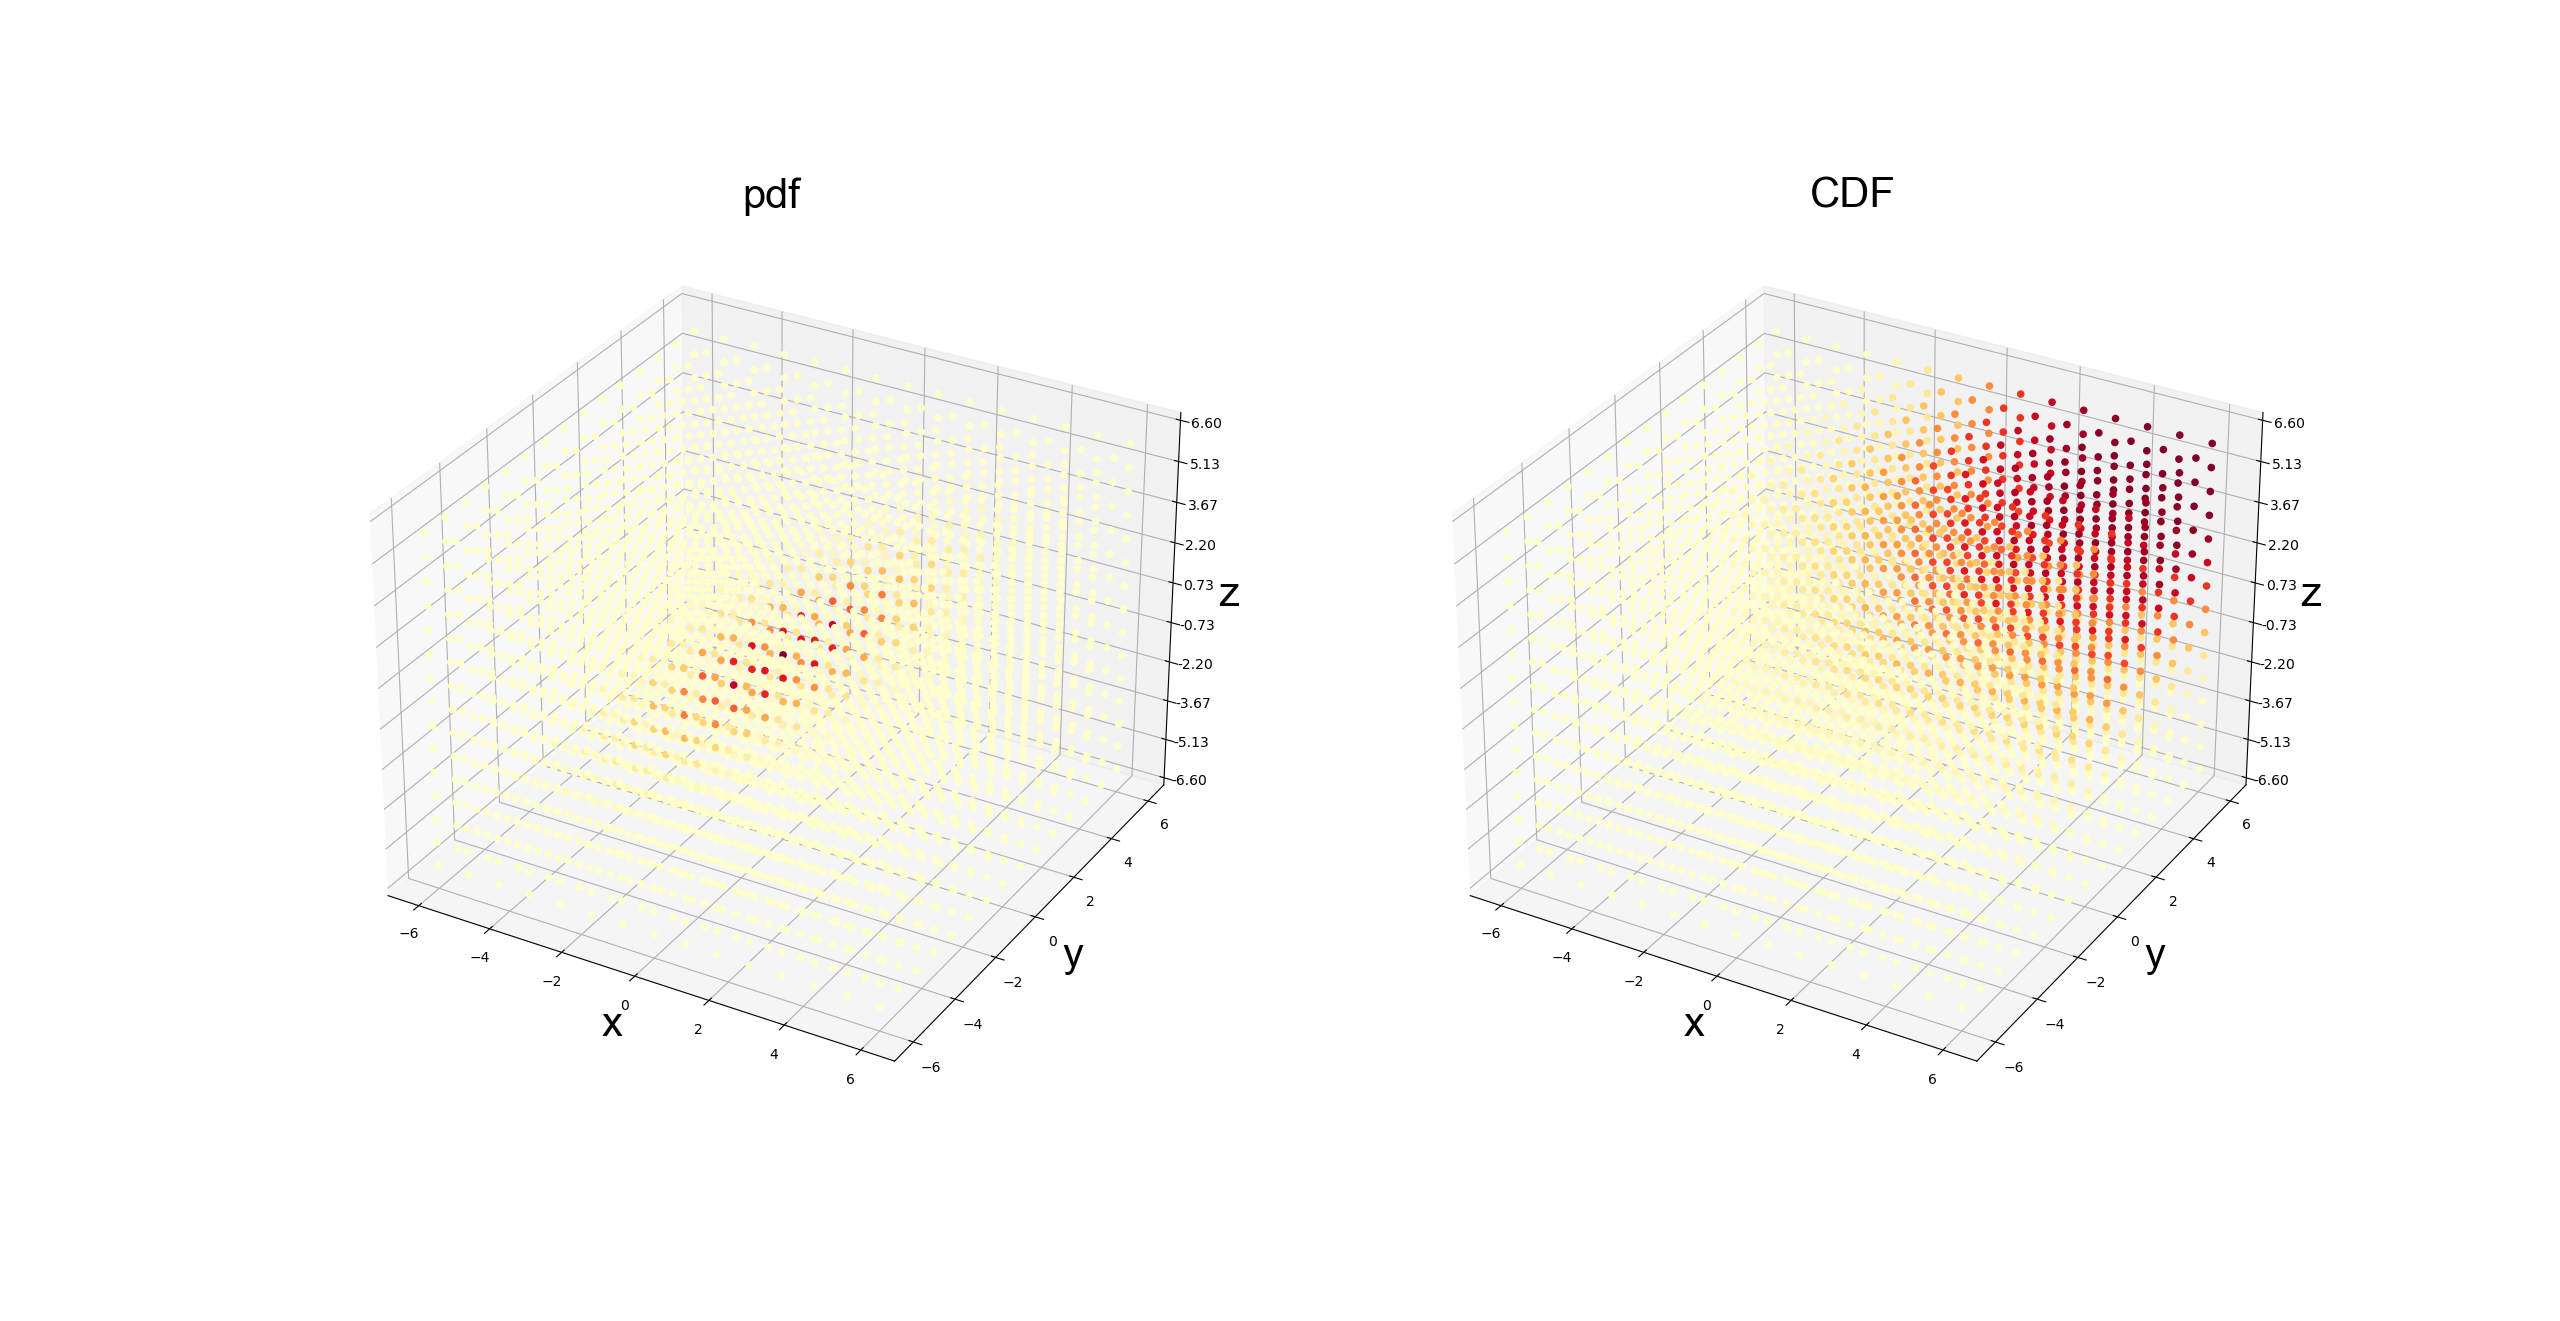
\includegraphics[height=6.5cm]{3D-3.png}
\end{frame}

 \section {Expectation Vectors and Covariance Matrices}
\begin{frame}
\frametitle{Expectation Vector}
The expectation of the vector $X=(X_1,...,X_n)^T$ is a vector $\mu = (\mu_1,..\mu_n)^T$ whose elements are given by:\newline\\
$\mu_i = \int_{-\infty}^{\infty}...\int_{-\infty}^{\infty} x_if_x(x_1,...,x_n)dx_1...dx_n.$\newline\\
$f_{X_i}(x_i) = \int_{-\infty}^{\infty}...\int_{-\infty}^{\infty} f_x(x)dx_1...dx_{i-1}dx_{i+1}...dx_n$\newline\\
$\mu_i=\int_{-\infty}^\infty x_if_{x_i}(x_i)dx_i$
\end{frame}

\begin{frame}
\frametitle{Covariance Matrix}
The covariance matrix associated with a real random vector$X$ is:\newline\\
$K = E[(X-\mu)(X-\mu)^T]$\newline\\
Define\newline\\
$K_{ij}= E[(X_i-\mu_i)(X_j-\mu_j)]$\newline\\
Particularly:
$\sigma_i^2=K_{ii}$, so we can write $K$ as:
$\begin{bmatrix}
   \sigma_1^2& ...&K_1n \\
    ...&\sigma_i^2&...\\
    K_{n1}&...&\sigma_n^2
\end{bmatrix}$\newline\\
1- if $X$ is real, all the elements of $K$ are *real*.\newline
2- $K_{ij}=K_{ji}$, the covariance matrix is *real symmetric*!\newline
3- Real symmetric matrices have many interesting properties! we will discuss it!\newline
\end{frame}

\begin{frame}
\frametitle{Correlation matrix}
The correlation matrix $R$ is defined by:\newline\\
$R=E[XX^T]$\newline\\
$R=R+\mu \mu^T$
, and\newline\\
$K=R-\mu\mu^T$\newline\\
\end{frame}

\begin{frame}
\frametitle{Definitions}
Consider real n-dimensional random vectors $X$, $Y$ with respective mean vectors $\mu_x, and \mu_y $:\newline\\
$X$, and $Y$ are *uncorrelated* if:\newline
$E[XY^T]=\mu_x\mu_y^T$\newline\\

$X$, and $Y$ are *orthogonal* if:\newline
$E[XY^T]=0$\newline\\

$X$, and $Y$ are *independent* if:\newline
$f_{XY}(x,y)=f_X(x)f_Y(y)$\newline

*Note: Independence implies uncorrelatedness! But the converse is not *generally* true!
\end{frame}

\begin{frame}
\frametitle{Expectation vector, Covariance matrix: Example!}
For vectors\newline $Y = (X_1,X_2)^T,\newline Z=(X_3,X_4)^T$,\newline we write their joint vector as\newline $X= (X_1,X_2,X_3,X_4)^T$\newline\\
and the joint PDF as:\newline\\
$f_X (x) = \frac{1}{4\pi^2}{exp(-\frac{1}{2}x^Tx)}$ \newline\\
Is this distribution familiar to you? \newline\\
let $\mu_Y$, and $\mu_Z$ be the mean vectors of vector $Y$, and $Z$ respectively,\newline\\
1- compute $\mu_Y$, and $\mu_Z$!, then $\mu_Y \mu_Z^T$
\end{frame}

\begin{frame}
\frametitle{Expectation vector, Covariance matrix: Example!}
$\mu_X=(\mu_1,\mu_2,\mu_3,\mu_4)$: the expectation of X vector, therefore\newline\\
$\mu_Y=(\mu_1,\mu_2), \mu_Z = (\mu_3,\mu_4)$\newline\\

$\mu_1 = \int_{-\infty}^{\infty}\int_{-\infty}^{\infty}\int_{-\infty}^{\infty} \int_{-\infty}^{\infty}  x_1f_x(x_1,x_2,x_3,x_4)dx_1dx_2dx_3dx_4$\newline\\
$\mu_1 = \int_{-\infty}^{\infty}\int_{-\infty}^{\infty}\int_{-\infty}^{\infty} \int_{-\infty}^{\infty}  x_1\frac{1}{4\pi^2}{exp(-\frac{1}{2}x^Tx)}dx_1dx_2dx_3dx_4 $ \newline\\
$\mu_1 = \frac{1}{4\pi^2} \int_{-\infty}^{\infty}\int_{-\infty}^{\infty}\int_{-\infty}^{\infty} \int_{-\infty}^{\infty} x_1exp(-\frac{1}{2}(x_1^2+x_2^2+x_3^2+x_4^2))dx_1dx_2dx_3dx_4 = 0$\newline\\
Therefore, $\mu_Y=\mu_Z=(0,0)^T$
$\mu_Y \mu_Z^T=
\begin{bmatrix}
    0&0 \\
0&0
\end{bmatrix}$
\end{frame}

\begin{frame}
\frametitle{Expectation vector, Covariance matrix: Example!}
 $Y = (X_1,X_2)^T$
 \newline $Z=(X_3,X_4)^T$,
 \newline $X= (X_1,X_2,X_3,X_4)^T$\newline\\
According to the previous part, $\mu_Y\mu_Z^T =\begin{bmatrix}
    0&0 \\
0&0
\end{bmatrix}
$
\newline\\
2- Compute $E(YZ^T)$!\newline\\
Are $Y$, and $Z$ orthogonal?
Are $Y$, and $Z$ uncorrelated?

\end{frame}

\begin{frame}
\frametitle{Expectation vector, Covariance matrix: Example!}
 $E(YZ^T) = \begin{bmatrix}
    EX_1X_3]&E[X_1X_4] \\
E[X_2X_3]&E[X_2X_4]
\end{bmatrix}$\newline\\

$E[X_1X_3]=  \int_{-\infty}^{\infty}\int_{-\infty}^{\infty}\int_{-\infty}^{\infty} \int_{-\infty}^{\infty}  x_1x_3exp(-\frac{1}{2}(x_1^2+x_2^2+x_3^2+x_4^2))dx_1dx_2dx_3dx_4=$ \newline\\ $\int_{-\infty}^{\infty}x_1exp(-\frac{1}{2}x_1^2)dx_1.\int_{-\infty}^{\infty}\int_{-\infty}^{\infty} \int_{-\infty}^{\infty}x_3exp(-\frac{1}{2}(x_2^2+x_3^2+x_4^2))dx_2dx_3dx_4 = 0$\newline\\
therefore, \newline\\

$E(YZ^T) = \begin{bmatrix}
    0&0 \\
0&0
\end{bmatrix}
 :$
$Y$, and $Z$ are orthogonal!\newline\\

$E(YZ^T) =\mu_Y\mu_Z^T$: 
$Y$, and $Z$ are uncorrelated!

\end{frame}



\begin{frame}
\frametitle{Expectation vector, Covariance matrix: Example!}
 $Y = (X_1,X_2)^T,\newline Z=(X_3,X_4)^T$,\newline $X= (X_1,X_2,X_3,X_4)^T$\newline\\
$f_X (x) = \frac{1}{4\pi^2}{exp(-\frac{1}{2}x^Tx)}$ \newline\\

3- Are $Y$, and $Z$ independent?
\end{frame}

\begin{frame}
\frametitle{Expectation vector, Covariance matrix: Example!}
$f_{YZ}(yz) = f_X (x) = \frac{1}{4\pi^2}{exp(-\frac{1}{2}x^Tx)} =$\newline\\ $\frac{1}{2\pi}exp(-\frac{1}{2}(x_1^2+x_2^2)).\frac{1}{2\pi}exp(-\frac{1}{2}(x_3^2+x_3^2)) =$ 
$f_Y(y)f_Z(z)$\newline\\
Therefore, $Y$, and $Z$ are independent!
\end{frame}

\begin{frame}
\frametitle{Expectation vector, Covariance matrix: Example!}
Compute the correlation matrix, $R$, and covariance matrix,$K$ for the joint vector, $X$!\newline\\
*reminder:\newline\\
$K = E[(X-\mu)(X-\mu)^T]$\newline
Define\newline
$K_{ij}= E[(X_i-\mu_i)(X_j-\mu_j)]$\newline
The correlation matrix $R$ is defined by:\newline
$R=E[XX^T]$\newline
$R=R+\mu \mu^T$
$K=R-\mu\mu^T$\newline\\

*hint! you will need it!
$\int_{-\infty}^{\infty}x^2exp(-ax^2)=\sqrt{\frac{\pi}{4a^3}}$
\end{frame}

\begin{frame}
\frametitle{Expectation vector, Covariance matrix: Example!}
Note that we have shown that $\mu_X=(0,0,0,0,0)^T$, therefore,\newline\\
$K=R-\mu\mu^T = R$\newline\\
and, $K_{ij}= E[(X_i-\mu_i)(X_j-\mu_j)] = E[X_iX_j]$\newline\\
and, we have shown that if $i\neq j: K_{ij}=E[X_iX_j] =0$\newline\\
So, we just need to compute $E[X_i^2]$, and since all variables are independent, and everything is symmetric, $E[X_1^2]=E[X_2^2]=E[X_3^2]=E[X_4^2]$
\end{frame}

\begin{frame}
\frametitle{Expectation vector, Covariance matrix: Example!}
$E[X_1^2] = \frac{1}{\sqrt{2*\pi}}\int_{-\infty}^{\infty} x_i^2exp(\frac{-1}{2}x_i^2).\frac{1}{\sqrt{{2*\pi}^2}}\int_{-\infty}^{\infty}\int_{-\infty}^{\infty}\int_{-\infty}^{\infty} exp(-\frac{1}{2}(x_2^2+x_3^2 +x_3^2)) dx_2dx_3dx_4 =$\newline\\
$\frac{1}{\sqrt{2*\pi}}\int_{-\infty}^{\infty} x_i^2exp(\frac{-1}{2}x_i^2).1 = \frac{\sqrt{2\pi}}{\sqrt{2\pi}}.1=1$\newline\\
So, $K =\begin{bmatrix}
   1&0&0&0 \\
   0&1&0&0\\
    0&0&1&0\\
    0&0&0&1
\end{bmatrix}$\newline\\

*Reminder
$\sigma_i^2=K_{ii}$, so we can write $K$ as:
$\begin{bmatrix}
   \sigma_1^2& ...&K_1n \\
    ...&K_{ii}^2&...\\
    K_{n1}&...&\sigma_n^2
\end{bmatrix}$\newline\\
\end{frame}

\begin{frame}
For both Y, and Z vectors, the PDF, is a multivariate Gaussian with:
\\mean, $\mu = [0,0]$,\\
covariance matrix $\Sigma = \begin{bmatrix}
    1 & 0 \\
    0&1
\end{bmatrix}$\newline\\
\frametitle{Expectation vector, Covariance matrix: Example!}
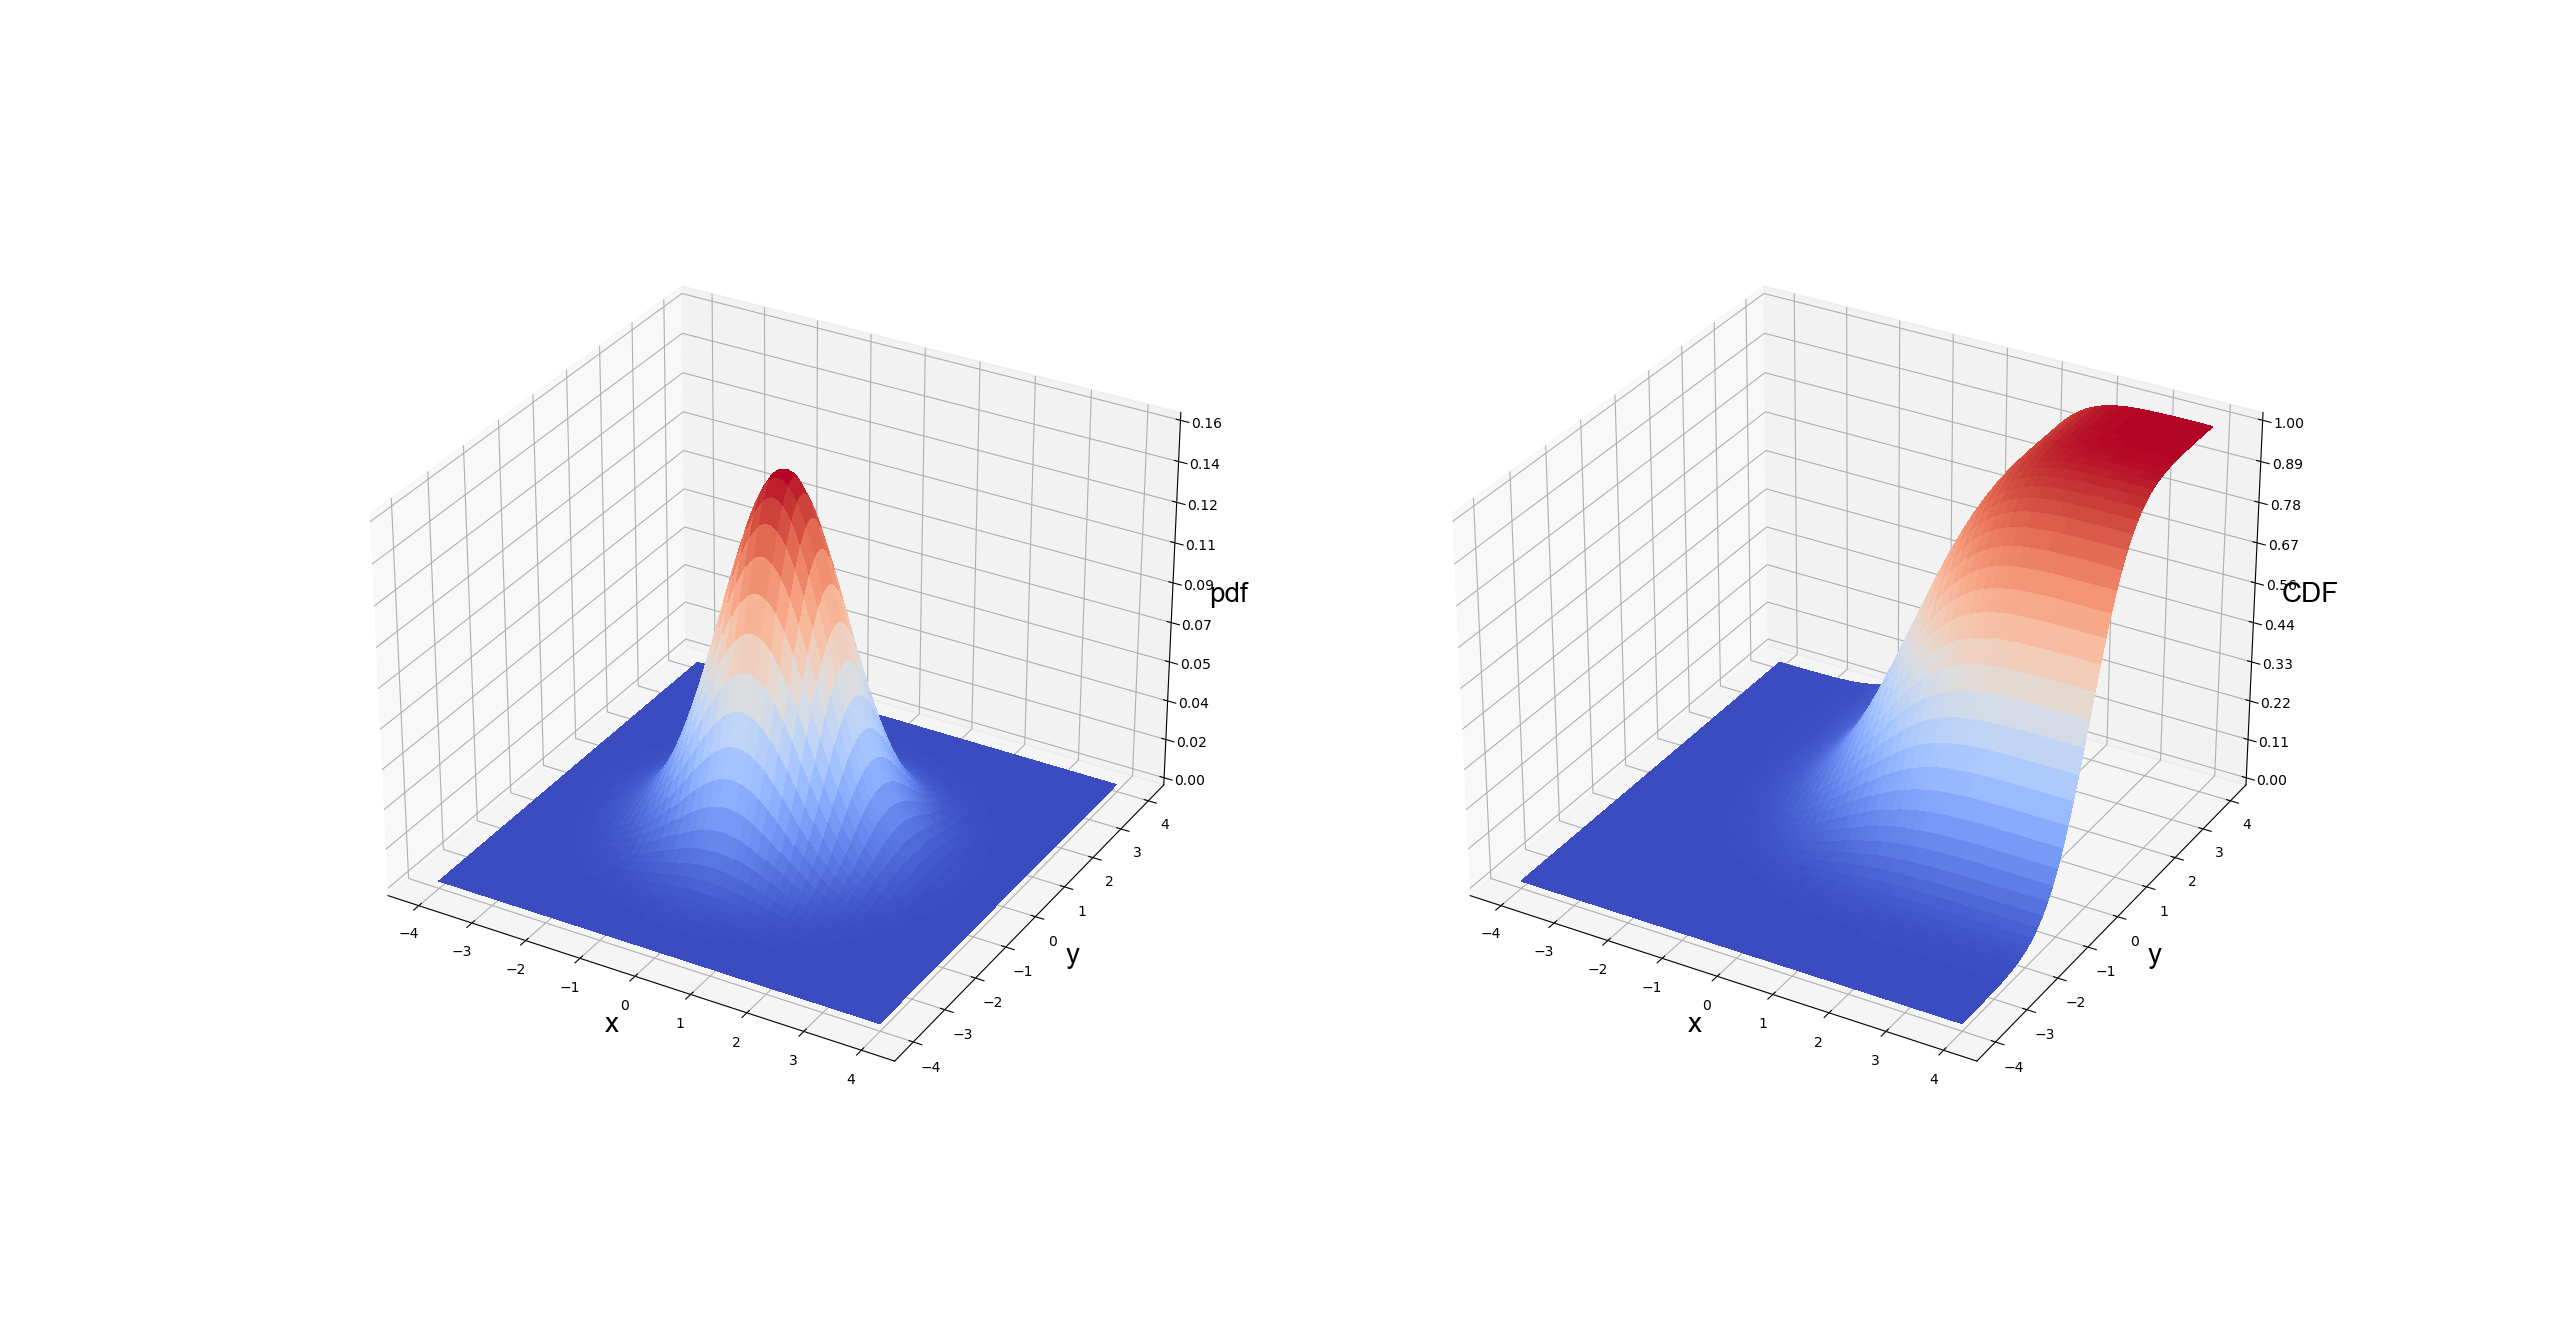
\includegraphics[height=6.5cm]{2D-1.png}
\end{frame}


\section{Properties of Covariance Matrices}
\begin{frame}
\frametitle{Properties of Covariance Matrices}
This is ...
\end{frame}

\section {The Multidimensional Gaussian Law}
\begin{frame}
\frametitle{The Multidimensional Gaussian Law}
This is ...
\end{frame}


 \section{Distribution of the Sample Mean}
\begin{frame}
\frametitle{Distribution of the Sample Mean}
This is ...
\end{frame}

 \section{Conditional Gaussian distributions }
\begin{frame}
\frametitle{Conditional Gaussian distributions}
This is ...
\end{frame}

 \section{Marginal Gaussian distributions }
\begin{frame}
\frametitle{Marginal Gaussian distributions}
This is ...
\end{frame}


\end{document}